\tikzset{bb/.style={draw, inner sep=2.5mm, rounded corners}}
\tikzset{
    ultra thin/.style= {line width=0.1pt},
    very thin/.style=  {line width=0.2pt},
    thin/.style=       {line width=0.4pt},
    semithick/.style=  {line width=0.6pt},
    thick/.style=      {line width=0.8pt},
    very thick/.style= {line width=1.2pt},
    ultra thick/.style={line width=1.6pt}
}

\begin{figure}
    \centering
    
    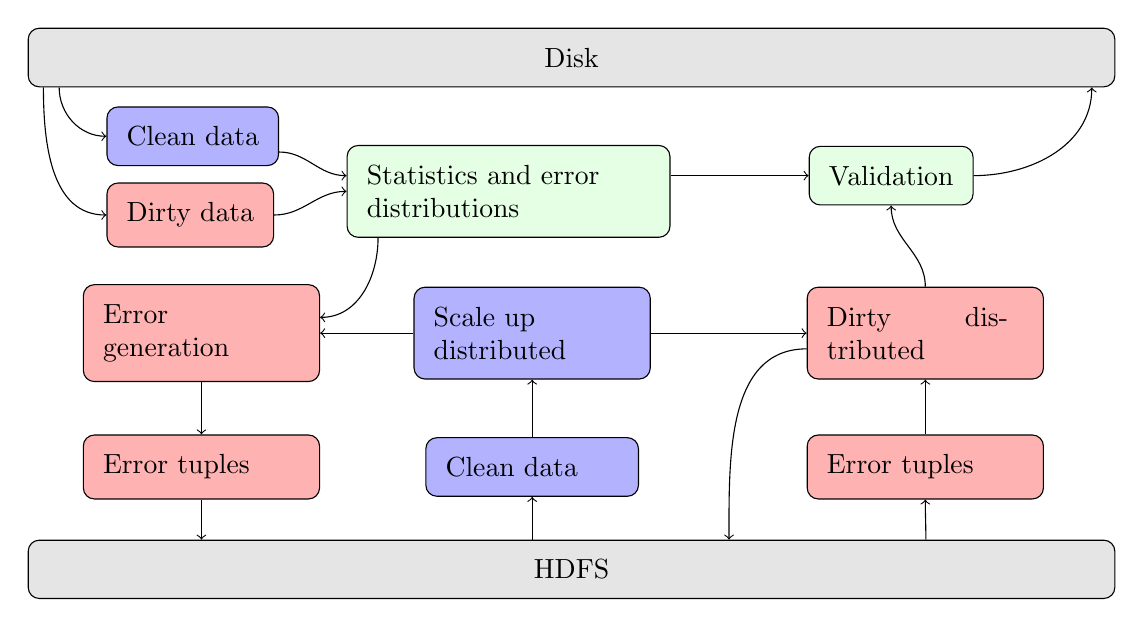
\begin{tikzpicture}[]
    \node[bb, text width=13.3cm, align = center, fill=black!10](disk){Disk};
    
    \node[bb, text width=13.3cm, align = center, fill=black!10] (hdfs) at ([yshift=-6.5cm] disk){HDFS};
    
    \node[bb, anchor = west, fill=blue!30] (clean) at ([yshift=-1.cm, xshift = 1cm] disk.west) {Clean data};
    \node[bb, anchor = west, fill=red!30] (dirty) at ([yshift=-2cm, xshift = 1cm] disk.west) {Dirty data};
    
    \node[bb, text width=2.2cm, fill=blue!30] (clean_dist) at ([yshift=-5.2cm, xshift = -0.5cm] disk) {Clean data};
    
    \node[bb, text width=3.6cm, fill=green!10] (stats) at ([yshift=-1.7cm, xshift = -0.8cm] disk) {Statistics and error distributions};
    
    \node[bb, text width=2.5cm, fill=blue!30] (scale_up) at ([yshift=-3.5cm, xshift = -0.5cm] disk) {Scale up \ \ \ \ \ \ \ \ \  distributed };
    
    \node[bb, text width=2.5cm, fill=red!30] (error_gen) at ([yshift=-3.5cm, xshift = -4.7cm] disk) {Error \ \ \ \ \ \ \ \ \ \ generation};
    \node[bb, text width=2.5cm, fill=red!30] (error_tuples) at ([yshift=-5.2cm, xshift = -4.7cm] disk) {Error tuples};
    
    % \node[bb, fill=red!30, text width=4.0cm, anchor = east] (errors) at ([yshift=-1.7cm,xshift= -0.8cm] disk.east) {Errors generation and introduction};
    
    \node[bb,  anchor=east, fill=green!10] (validation) at ([yshift=-1.5cm, xshift=-1.8cm] disk.east) {Validation};
    
    \node[bb,  anchor=east, fill=red!30, text width = 2.5cm] (dirty_dist) at ([yshift=-3.5cm, xshift=6cm] disk) {Dirty \ \ \ \ \ \ \ distributed};
    
    \node[bb, anchor=east, text width=2.5cm, fill=red!30] (error_tuples_out) at ([yshift=-5.2cm, xshift = 6cm] disk) {Error tuples};
    
    
    \draw[->] ([xshift=0.4cm]disk.south west) to[out = -90, in = 180] (clean);
    \draw[->] ([xshift=-0.5cm]hdfs.north) to[out = 90, in = -90] (clean_dist);
    \draw[->] ([xshift=0.0cm]clean_dist.north) to[out = 90, in = -90] (scale_up);
    \draw[->] ([xshift=0.2cm]disk.south west) to[out = -90, in = 180] (dirty);
    
    \draw[->] ([xshift=0.4cm, yshift=-0.0cm]stats.south west) to[out = -90, in = 0] ([yshift=0.2cm]error_gen.east);
    \draw[->] ([yshift=-0.0cm]scale_up.west) to[out = 180, in = 0] ([yshift=-0.0cm]error_gen.east);
    \draw[->] ([xshift=0.0cm]error_tuples.south) to[out = -90, in = 90] ([xshift=-4.7cm]hdfs.north);
    \draw[->] ([xshift=0.0cm]error_gen.south) to[out = -90, in = 90] ([xshift=0cm]error_tuples.north);
    
    % \draw[->] ([]clean.east) to[out = 0, in = 180] (scale_up);
    
    \draw[->] ([yshift=-0.2cm]clean.east) to[out = 0, in = 180] ([yshift=0.2cm] stats.west);
    
    \draw[->] ([]dirty.east) to[out = 0, in = 180] (stats);
    
    % \draw[->] ([]scale_up.east) to[out = 0, in = 180] (errors);
    
    % \draw[->] ([]stats.east) to[out = 0, in = -90] ([xshift=0.2cm]errors.south west);
    
    % \draw[->] ([]errors.east) to[out = 30, in = -90] ([xshift=-0.5cm]disk.south east);
    
    \draw[->] ([]validation.east) to[out = 0, in = -90] ([xshift=-0.3cm]disk.south east);
    
    % \draw[->] ([xshift=-0.8cm]errors.south) to[out = -90, in = 180] ([]validation.west);
    
    \draw[->] ([yshift=0.2cm]stats.east) to[out = 0, in = 180] ([yshift=-0.0cm]validation.west);
    
    \draw[->] ([xshift=4.5cm]hdfs.north) to[out = 90, in = -90] (error_tuples_out);
    
    \draw[->] ([xshift=0cm]error_tuples_out.north) to[out = 90, in = -90] (dirty_dist);
    
    \draw[->] ([xshift=0cm]scale_up.east) to[out = 0, in = 180] (dirty_dist.west);
    
    \draw[->] ([yshift=-0.2cm]dirty_dist.west) to[out = 180, in = 90] ([xshift=2cm]hdfs.north);
    
    \draw[->] ([yshift=0cm]dirty_dist.north) to[out = 90, in = -90] ([xshift=0cm]validation.south);
    
    \end{tikzpicture}
    
    \caption{\label{fig:data_gen_dist}Distributed data generator}
    
\end{figure}